%
% Enkonduko por Unua Libro
%

% Ni facile povas difini papergeometrio.
%
\usepackage[a5paper,margin=2cm]{geometry}

% Creative Commons icons
%
\usepackage{ccicons}

% preciza substreko
% 
\usepackage{soul}

% datoprezento angla kaj esperanta
%
\def\mytoday{\number\day \space \ifcase\month\or January\or February\or March\or April\or May\or June\or July\or August\or September\or October\or November\or December\fi \space \number\year}
\def\hodiau{\number\day a~de~\ifcase\month\or januaro\or februaro\or marto\or aprilo\or majo\or junio\or julio\or aŭgusto\or septembro\or oktobro\or novembro\or decembro\fi, \number\year}

% Ni bezonas germanajn citilojn, kiam demanditaj.
%
\usepackage[english]{babel}  

% Por ornamoj kiel la "por angloj" etikedo; beletaj sekcilineoj
%
\usepackage{pgfornament} 

% La ornamaĵoj de la "por angloj" etikedo
%
\makeatletter\newcommand{\anglojcurlicue}{%
\begingroup
\def\i{\pgfusepath{clip}}%
\let\o\pgfpathclose
\let\s\pgfusepathqfillstroke
\def\p ##1##2{\pgfqpoint{##1bp}{##2bp}}%
\def\m ##1 ##2 {\pgfpathmoveto{\p{##1}{##2}}}%
\def\l ##1 ##2 {\pgfpathlineto{\p{##1}{##2}}}%
\def\r ##1 ##2 ##3 ##4 {\pgfpathrectangle{\p{##1}{##2}}{%
                       \p{##3}{##4}}}%
\def\c ##1 ##2 ##3 ##4 ##5 ##6 {%
\pgfpathcurveto{\p{##1}{##2}}{\p{##3}{##4}}{\p{##5}{##6}}}%
\m 358.457 422.057 
\c 361.672 422.043  364.859 421.978  367.958 421.027 
\c 368.436 420.881  368.863 420.604  369.316 420.393 
\c 377.517 418.72  382.067 410.126  382.226 401.945 
\c 382.226 392.003  374.167 383.944  364.226 383.945 
\c 354.284 383.944  346.226 392.003  346.226 401.945 
\c 346.398 405.355  347.048 408.821  349.141 411.625 
\c 343.415 409.233  345.878 410.48  341.65 408.097 
\c 324.998 397.034  318.678 382.874  313.275 364.023 
\l 313.275 342.647 
\c 316.649 345.968  320.675 348.491  324.663 350.99 
\c 324.85 351.1  325.038 351.209  325.226 351.317 
\c 334.609 356.375  344.634 359.71  355.399 359.766 
\l 355.399 359.766 
\c 357.713 359.67  360.035 359.697  362.341 359.478 
\c 368.372 358.907  374.295 357.501  380.014 355.532 
\c 394.271 350.6  407.757 342.194  424.366 329.183 
\c 428.505 325.941  441.463 315.402  443.489 313.801 
\c 449.676 308.91  453.925 305.949  457.145 304.339 
\c 459.514 303.345  458.529 303.582  460.001 303.305 
\c 458.843 306.045  458.197 307.848  458.226 310.945 
\c 458.226 320.886  466.284 328.944  476.226 328.945 
\c 486.167 328.944  494.226 320.886  494.226 310.945 
\c 494.127 308.987  494.255 309.706  494.063 308.761 
\c 494.683 302.4  491.182 296.358  487.77 291.296 
\c 479.433 279.687  462.059 277.285  447.306 284.661 
\c 442.377 287.126  437.142 290.775  429.846 296.542 
\c 427.646 298.281  414.738 308.778  410.8 311.864 
\c 408.104 313.954  405.417 316.064  402.638 318.042 
\c 402.518 312.06  402.812 314.75  402 309.948 
\c 397.477 292.939  383.713 282.479  366.133 282.107 
\c 365.464 281.971  366.089 282.094  364.226 282 
\c 354.284 282  346.226 290.059  346.226 300 
\c 346.226 309.941  354.284 318  364.226 318 
\c 372.76 317.569  380.302 312.101  381.819 303.379 
\c 384.424 306.198  386.602 309.286  387.346 313.149 
\c 389.374 322.434  383.942 331.049  370.298 335.471 
\l 369.84 335.672 
\c 368.378 336.045  366.933 336.489  365.454 336.79 
\c 355.382 338.839  345.099 337.455  336.176 332.235 
\c 336.047 332.161  335.916 332.089  335.788 332.01 
\c 323.801 324.574  316.722 319.893  313.275 305.317 
\l 313.275 280.457 
\l 294.275 280.457 
\l 294.275 310.52 
\c 291.099 320.797  281.841 326.621  273.212 332.011 
\c 273.084 332.089  272.953 332.161  272.824 332.235 
\c 263.901 337.455  253.618 338.839  243.546 336.79 
\c 242.067 336.489  240.622 336.045  239.16 335.672 
\l 238.702 335.471 
\c 225.058 331.049  219.626 322.434  221.654 313.149 
\c 222.398 309.286  224.576 306.198  227.181 303.379 
\c 228.698 312.101  236.24 317.569  244.774 318 
\c 254.716 318  262.775 309.941  262.775 300 
\c 262.775 290.059  254.716 282  244.775 282 
\c 242.911 282.094  243.536 281.971  242.867 282.107 
\c 225.287 282.479  211.523 292.939  207 309.948 
\c 206.188 314.75  206.482 312.06  206.362 318.042 
\c 203.583 316.064  200.896 313.954  198.2 311.864 
\c 194.262 308.778  181.354 298.281  179.154 296.542 
\c 171.858 290.775  166.623 287.126  161.694 284.661 
\c 146.941 277.285  129.567 279.687  121.23 291.296 
\c 117.818 296.358  114.317 302.4  114.938 308.761 
\c 114.745 309.706  114.873 308.987  114.775 310.945 
\c 114.775 320.886  122.833 328.944  132.775 328.944 
\c 142.716 328.944  150.775 320.886  150.775 310.944 
\c 150.803 307.848  150.157 306.045  148.999 303.305 
\c 150.471 303.582  149.486 303.345  151.855 304.339 
\c 155.075 305.949  159.324 308.91  165.511 313.801 
\c 167.537 315.402  180.495 325.941  184.634 329.183 
\c 201.243 342.194  214.729 350.6  228.986 355.532 
\c 234.705 357.501  240.628 358.907  246.659 359.478 
\c 248.965 359.697  251.287 359.67  253.601 359.766 
\l 253.601 359.766 
\c 264.366 359.71  274.391 356.375  283.774 351.317 
\c 283.962 351.209  284.15 351.1  284.337 350.99 
\c 287.81 348.892  291.248 346.678  294.275 343.953 
\l 294.275 369.085 
\c 290.119 384.973  280.964 398.898  267.35 408.097 
\c 263.122 410.48  265.585 409.233  259.859 411.625 
\c 261.952 408.821  262.602 405.355  262.774 401.945 
\c 262.775 392.003  254.716 383.944  244.774 383.944 
\c 234.833 383.944  226.774 392.003  226.774 401.944 
\c 226.933 410.126  231.484 418.72  239.684 420.393 
\c 243.116 422.384  248.167 421.843  252.047 422.133 
\l 252.047 422.133 
\c 259.298 422.061  265.828 419.236  272.058 415.768 
\c 281.705 410.074  288.522 401.42  294.275 392.033 
\l 294.275 421.284 
\c 289.186 424.522  286.795 430.165  286.5 436 
\c 286.589 441.902  289.361 447.399  294.275 450.716 
\l 294.275 517.457 
\c 295.916 521.406  297.782 528.367  302.297 530.098 
\c 302.804 530.292  303.371 530.257  303.908 530.337 
\c 309.147 529.012  311.696 522.196  313.275 517.457 
\l 313.275 451.696 
\c 319.102 448.288  322.164 442.654  322.5 436 
\c 322.156 428.426  319.388 424.432  313.275 420.304 
\l 313.275 389.526 
\c 318.642 400.29  327.107 409.021  336.942 415.768 
\c 343.172 419.236  349.702 422.061  356.953 422.133 
\s
\endgroup}
\makeatother

% interlinea distanco
%
\usepackage{setspace} 

% beletaj ombroj por ornamoj tiparoj
%
\usepackage{shadowtext}
\shadowoffset{1pt}

% la "R" en "Dr." je la titolpaĝo
%
\usepackage{stackengine}  

% star lines in poems
% 
\newcommand{\pstars}{%
\hspace*{\fill} * \hspace{3em} \raisebox{-1em}{*} \hspace{3em} * \hspace*{\fill}}

% la klasika montra fingro, kiu ekkrius "19a jarcento" se ĝi povus
%
\usepackage{dingbat}

% ŝanĝas la grando de la intermorgema signeto por ĝia kunteksto
%
\usepackage{relsize} 

% la krommarĝeno por la unua lineo de ĉiu alineo devus esti kiel la aliaj
%
\usepackage{indentfirst} 

% URLoj en la komento pri komposti
%
\usepackage{hyperref}

% la krommarĝeno por unuobla alineo
%
\usepackage{changepage}

% horitontala formato kaj pluraj kolonoj por la vortaro
%
\usepackage{pdflscape}
\usepackage{multicol}

% la xelatex-simbolo en la kompostanta komento
%
\usepackage{dtk-logos}

% granda longa tablo (la "mi ne scias ..." analizo)
%
\usepackage{longtable}

% tabularx helpos meti la Promesoj, kaj difinas la larĝeco de niaj tabloj
% 
\usepackage{tabularx}

% jen kolona spico "Y", kiu centras tabularx-ajn "X" kolonojn
% 
\newcolumntype{Y}{>{\centering\arraybackslash}X}

% por la longaj krampoj en la "Mi ne scias" tablo, kaj la vortara
% lineoj de "la" kaj "l'"
%
\usepackage{multirow} 

% por la belaj tiparoj
%
\usepackage{fontspec}

% el Google Fonts
\setmainfont{Old Standard TT}
\newfontfamily\cowboyfont{Smokum}[LetterSpace=5]
\newfontfamily\fjallafont{FjallaOne}
\newfontfamily\grammarpartsfont{FjallaOne}[LetterSpace=20]

% en MacOS
\newfontfamily\didone{Didot}
\newfontfamily\copper{Copperplate Light}[LetterSpace=5]

% el Font Squirrel
\newfontfamily\latinia{Latinia}

% el dafont
\newfontfamily\monastic{K22 Monastic}
\newfontfamily\bosox{Bosox}

% el Liberation Fonts
\newfontfamily\sansfont{Liberation Sans}[LetterSpace=5]

% sans-serif bolds in body text
%
\newcommand\inbold[1]{\scalebox{1}[0.8]{\fjallafont{#1}}}

% titlesec -- better section/chapter headings
%
\usepackage[compact,center]{titlesec}
\titlespacing*{\chapter}{0pt}{6em}{0pt}

% nice section heading for Patro Nia, etc.
%
\newcommand\secthead[3]{%
\vspace{#2}

{\hfil \scalebox{1.6}[1]{\didone{\bf #1}}}

\vspace{#3}}

% fancy page headers, that is, in imitation of the original
%
\usepackage{fancyhdr}
\setlength{\headheight}{15pt}
\pagestyle{fancy}

\fancyhf{}

% remove the rule at top of page
%
\renewcommand{\headrulewidth}{0pt}

% letters in the alphabet table at end of book
%
\newcolumntype{+}{>{\global\let\currentrowstyle\relax}}
\newcolumntype{^}{>{\currentrowstyle}}
\newcommand{\rowstyle}[1]{\gdef\currentrowstyle{#1}%
#1\ignorespaces
}

% index finger
%
\newcommand\finger{\raisebox{-0.5ex}{\Large \leftpointright \hspace{1em}}}

% this bit removes the page number from the chapter start page
%
\fancypagestyle{plain}{%
  \renewcommand{\headrulewidth}{0pt}%
  \fancyhf{}%
}

% pgfornament line to end a section
%
\newcommand{\sectionline}{
\begin{center}
\pgfornament[width=0.5\textwidth]{89}
\end{center}}

% la "por angloj" etikedo
%
\sodef\angloj{}{.2em}{0.6em}{0pt}
\newcommand{\poranglojbox}{%
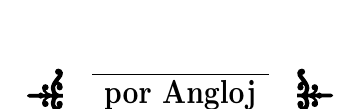
\begin{tikzpicture}[every node/.style={inner sep=0pt}]
\node[align=center](Text){\scalebox{1}[1.2]{\didone{\bf\angloj{por Angloj}}}} ;
\node[shift={(5pt,2pt)},anchor=center](CNW) at (Text.north east) {};
\node[shift={(-5pt,2pt)},anchor=center](CNE) at (Text.north west) {};
\node[shift={(-5pt,-2pt)},anchor=center](CSW) at (Text.south west) {};
\node[shift={(5pt,-2pt)},anchor=center](CSE) at (Text.south east) {};
\draw(CNW) to (CNE);
\draw(CSW) to (CSE);
\pgftransformshift{\pgfpoint{-1cm}{-0.537cm}}
\pgftransformscale{0.05};
\pgftransformrotate{90};
\anglojcurlicue{};
\pgftransformreset;
\pgftransformshift{\pgfpoint{1cm}{0.537cm}}
\pgftransformscale{0.05};
\pgftransformrotate{-90};
\anglojcurlicue{};
\end{tikzpicture}}

% the command for the morpheme-separation stroke
%
\renewcommand{\,}{%
{\relsize{-2.5}\raisebox{-1.35ex}{$'$}}}

% displays the "R." in "DR." on the title page raised and underlined
%
\newcommand{\doktoror}{\setul{3pt}{.4pt}\setbox0=\hbox{X}\belowbaseline[-\ht0]{\ul{\small R.}}}

% kapliteroj por la Vortaro
% 
\newcommand{\vorhead}[1]{\vspace{1.5ex}
{\hfil \scalebox{1.5}[1]{\sansfont{#1}}}
\vspace{1.5ex}}

\newenvironment{outdent}[1]
  {\setlength{\leftskip}{#1}%%
   \setlength{\parindent}{-#1}%%
  }
  {\par}

%
% generate the front of a Promeso card
%
\setlength{\fboxrule}{1.8pt}

\newcommand{\promeso}{%
\fbox{%
\begin{minipage}[t][3in]{0.4\linewidth}
\mbox{}
\begin{center}
\vspace{-2ex}
\scalebox{1.2}[1]{\didone{\textbf{Promes\,o.}}}
\end{center}

{\setlength{\parindent}{2.5em}

Mi, sub\,skrib\,it\,a, pro\-mes\,as el\,ler\-n\,i la pro\-pon\,it\,a\,n de d-r\,o \mbox{Esperanto} ling\-v\,o\,n in\-ter\,na\-ci\,a\,n, se est\,os montr\,it\,a, ke dek mi\-li\-on\,o\,j per\-son\,o\,j don\,is pub\-lik\,e ti\-a\,n sa\-m\,a\,n pro\-mes\,o\,n.

\paragraph{}
\textit{Sub\,skrib\,o:}}
\end{minipage}}}

% generate the back of a Promeso card
%
\newcommand{\nomadreso}{%
\fbox{%
\begin{minipage}[t][3in]{0.4\linewidth}
\mbox{}

{\setlength{\parindent}{0.5em}
\textbf{Nom\,o:}

\vspace{4ex}

\textbf{Adres\,o:}}

\end{minipage}}}

% Big delimiters in the demo sentence table
%
\newcommand{\tlba}{\scalebox{1}[1.25]\{}
\newcommand{\trba}{\scalebox{1}[1.25]\}}
\newcommand{\tlbb}{\multirow{2}{*}{\scalebox{1}[2.5]\{}}
\newcommand{\trbb}{\multirow{2}{*}{\scalebox{1}[2.5]\}}}
\newcommand{\tlbc}{\multirow{3}{*}{\scalebox{1}[4]\{}}
\newcommand{\trbc}{\multirow{3}{*}{\scalebox{1}[4]\}}}

